% PDF build: latex -> bibtex -> latex -> dvips -> ps2pdf
\documentclass[11pt,a4paper]{article}
\usepackage{amsmath,amsfonts,amssymb,graphicx,hyperref,xcolor,multicol,lipsum}
\usepackage[bahasa,english]{babel}
\usepackage[square]{natbib}             % bibliography style package

\bibpunct{(}{)}{;}{a}{}{,}              % bibliography style format:
                                        %         author [year]
\hypersetup{colorlinks=true,allcolors=blue}

\title{Judul and Title: Bilingual Paper}
\author{\textit{P. E. Nulis} \and \textit{A. U. Thor}}
\date{\today}

\begin{document}
\selectlanguage{bahasa} % by default, using last item in list [bahasa,english]
\maketitle

\begin{abstract}
\lipsum[1]
\end{abstract}

\begin{multicols}{2}

\section{Introduction}
\lipsum

\section{Data}
\lipsum

\end{multicols}

\begin{figure}
    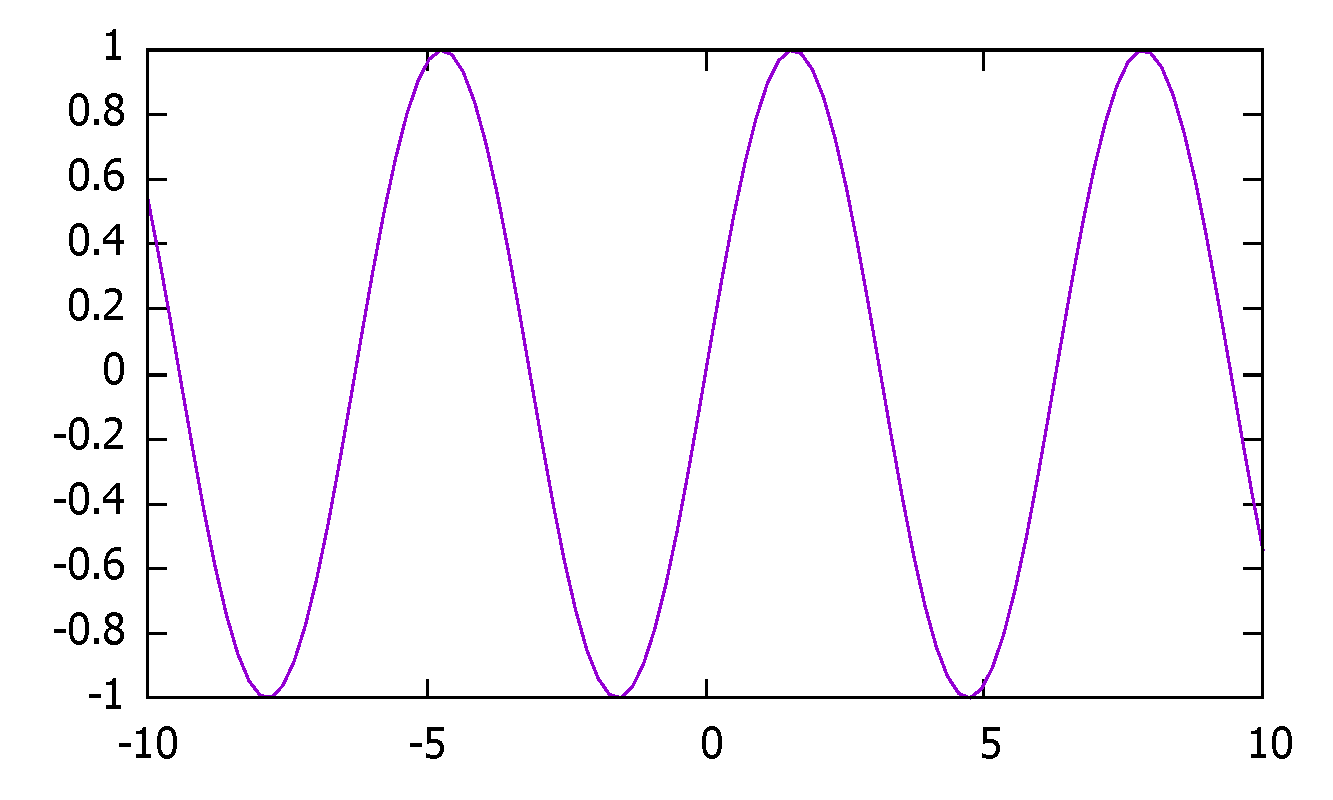
\includegraphics[width=\linewidth]{plot}
    \caption[Plot of $\sin x$.]{Plot of $\sin x$.}
    \label{fig:plot}
\end{figure}

\begin{multicols}{2}

\section{Result}
\lipsum\ As you can refer to \cite{siess2000} and \cite{stepien2002}.

\section{Conclusion}
\lipsum

\section*{Acknowledgement}
\lipsum[4]

\bibliography{makalah}
\bibliographystyle{authordate1}

\end{multicols}

\end{document}